\noindent

\includegraphics[height=1.25cm]{images/pictograms/benchmark}

\includegraphics[height=1.25cm]{images/pictograms/FEM}

\includegraphics[height=1.25cm]{images/pictograms/3d}

\includegraphics[height=1.25cm]{images/pictograms/paraview}

%%%%%%%%%%%%%%%%%%%%%%%%%%%%%%%%%%%%%%%%%%%%%%%%%%%%%%%%%%%%%%%%%%%%%%%%%%%%%%%%%%%%%%%%%%%%%%%%%%%

\begin{flushright} {\tiny {\color{gray} python\_codes/fieldstone\_82/text.tex}} \end{flushright}

%\lstinputlisting[language=bash,basicstyle=\small]{python_codes/fieldstone_82/keywords.key}

\par\noindent\rule{\textwidth}{0.4pt}

\begin{center}
\inpython
{\small Code: \url{https://github.com/cedrict/fieldstone/tree/master/python_codes/fieldstone_82}}
\end{center}

\par\noindent\rule{\textwidth}{0.4pt}

Last revision: October 13th, 2025.

\par\noindent\rule{\textwidth}{0.4pt}

%%%%%%%%%%%%%%%%%%%%%%%%%%%%%%%%%%%%%%%%%%%%%%%%%%%%%%%%%%%%%%%%%%%%%%%%%%%%%%%%%%%%%%%%%%%%%%%%%%%

The basis functions for this element is presented in Section~\ref{MMM-ss:Q1Q1bb_3D}.
This element is presented in \textcite{kahp20} (2020). 

There are two bubble functions/nodes per element so we then have 
\begin{lstlisting}
nn_V=nnx*nny*nnz+2*nel 
nn_P=nnx*nny*nnz
\end{lstlisting}
For a $8\times 8 \times 8=512$ element grid, there are $9^3=729$ nodes, and 1024 bubble nodes.
We then have $3\cdot 729=2157$ $Q_1$ velocity dofs and 3072 velocity dofs attached 
to the bubbles.
Since the bubble nodes are stored last the structure of the matrix is as follows:
\begin{center}
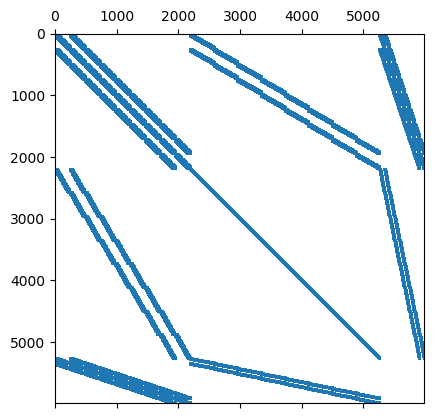
\includegraphics[width=7cm]{python_codes/fieldstone_82/RESULTS/matrix_8x8x8_bef_bc}
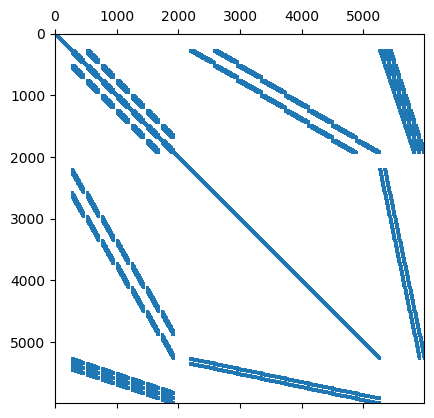
\includegraphics[width=7cm]{python_codes/fieldstone_82/RESULTS/matrix_8x8x8_aft_bc}\\
{\captionfont Sparsity pattern of the matrix for a 8x8x8 grid.
nn\_V=1753, nn\_P=729.\\ Left:
before boundary conditions are applied. 
Right: after boundary conditions are applied.} 
\end{center}

Note that the matrix building and assembly could be carried out 
much faster as documents in stone 182 for example.
The solve strategy is as follows: either the matrix is built 
as a whole (see figures above) and passed to the (direct) solver
(with or without Reversed Cuthill McKee reordering), 
either the $\K$ and $\G$ blocks are built separately and 
a Schur complement conjugate gradient solver is used (see benchmark 5). 

%......................................
\subsection*{Manufactured solution (bench=1)}

This benchmark begins by postulating a polynomial solution 
to the 3D Stokes equation (see Dohrmann \& Bochev (2004) \cite{dobo04}):
\begin{equation}
\vec{\upnu}(x,y,z)
=
\left(
\begin{array}{c}
x+x^2+xy+x^3y \\
y + xy + y^2 + x^2 y^2\\
-2z - 3xz - 3yz - 5x^2 yz
\end{array}
\right)
\label{eqbur2}
\end{equation}
and
\begin{equation}
p(x,y,z) = xyz + x^3 y^3z - 5/32
\end{equation}
The corresponding right-hand side is computed in Section~\ref{MMM-mms_db3D}.
The domain is a unit cube and velocity boundary conditions
simply use Eq.~\eqref{eqbur2}.
Note that the pressure fulfills $\int_\Omega p(x,y,z) dV = 0.$

\begin{center}
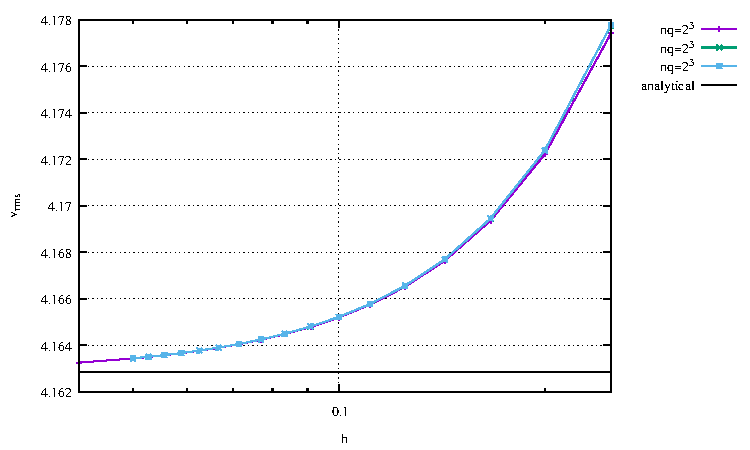
\includegraphics[width=8cm]{python_codes/fieldstone_82/RESULTS/bench1/vrms.pdf}
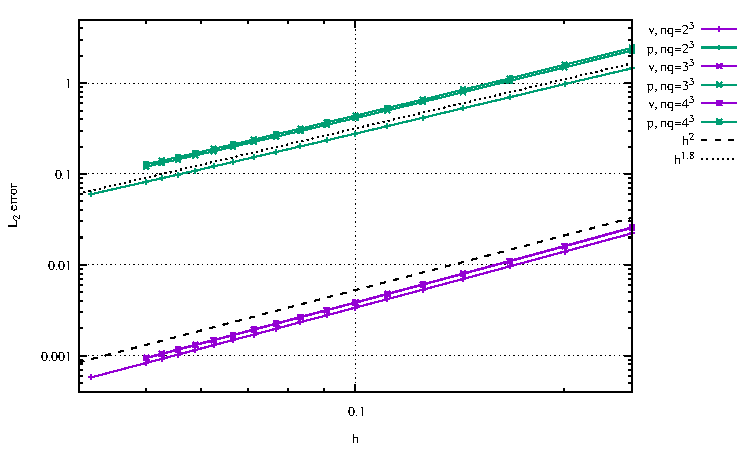
\includegraphics[width=8cm]{python_codes/fieldstone_82/RESULTS/bench1/conv.pdf}\\
{\captionfont Results obtained for three levels of quadrature, with $\beta=0$ (i.e.
viscosity is constant and equal to 1).}
\end{center}

Somewhat surprisingly, the pressure convergence is not exactly quadratic but seems to be
around 1.8. Also, the $2\times 2\times 2$ 
quadrature yields better results than the $3\times 3\times 3$ or $4\times 4 \times 4$.

\newpage
%......................................
\subsection*{Horizontal shear (bench=2)}

This is a simple kinematical test: gravity is set to zero, 
Viscosity is 1.
The analytical solution $(u,v,w)=(0.5-z,0,0)$ is prescribed on all sides. 
The analytical pressure solution is $p=0$.
The root mean square velocity is then
\[
\upnu_{rms}
=\sqrt{ \frac{1}{L_xL_yL_z} \iiint_\square (u^2+v^2+w^2)dxdydz }
=\sqrt{ \int_0^1 (\frac12-z)^2dz  }
\simeq 0.288675
\]

\begin{center}
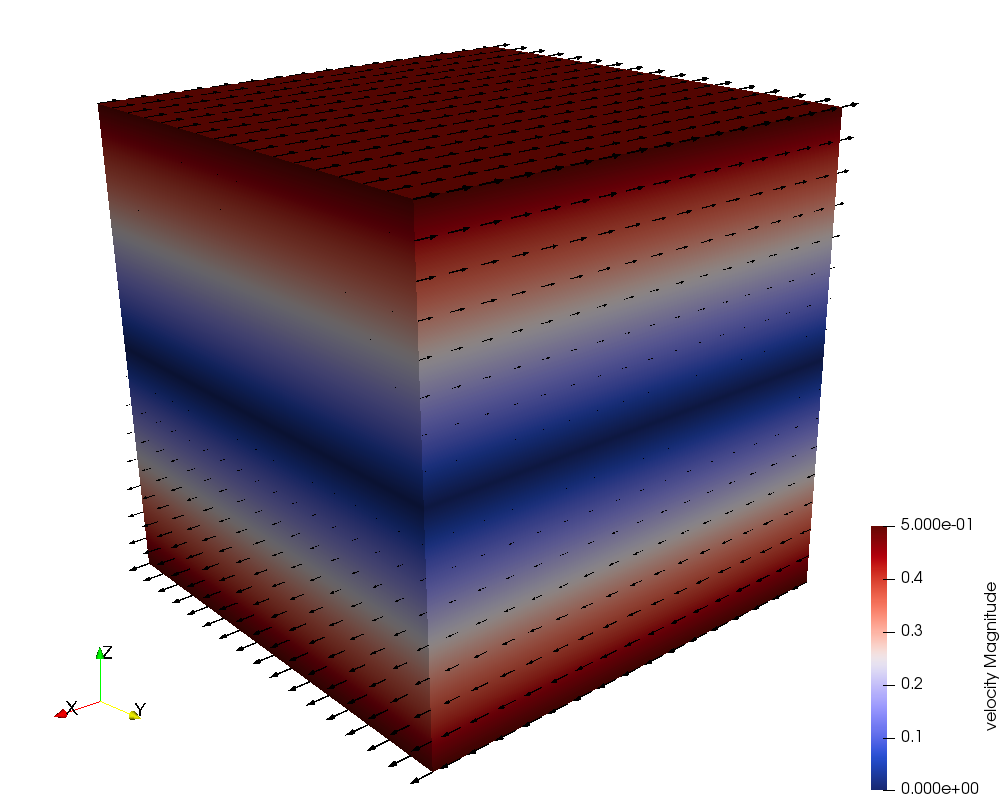
\includegraphics[width=5cm]{python_codes/fieldstone_82/RESULTS/bench2/vel}
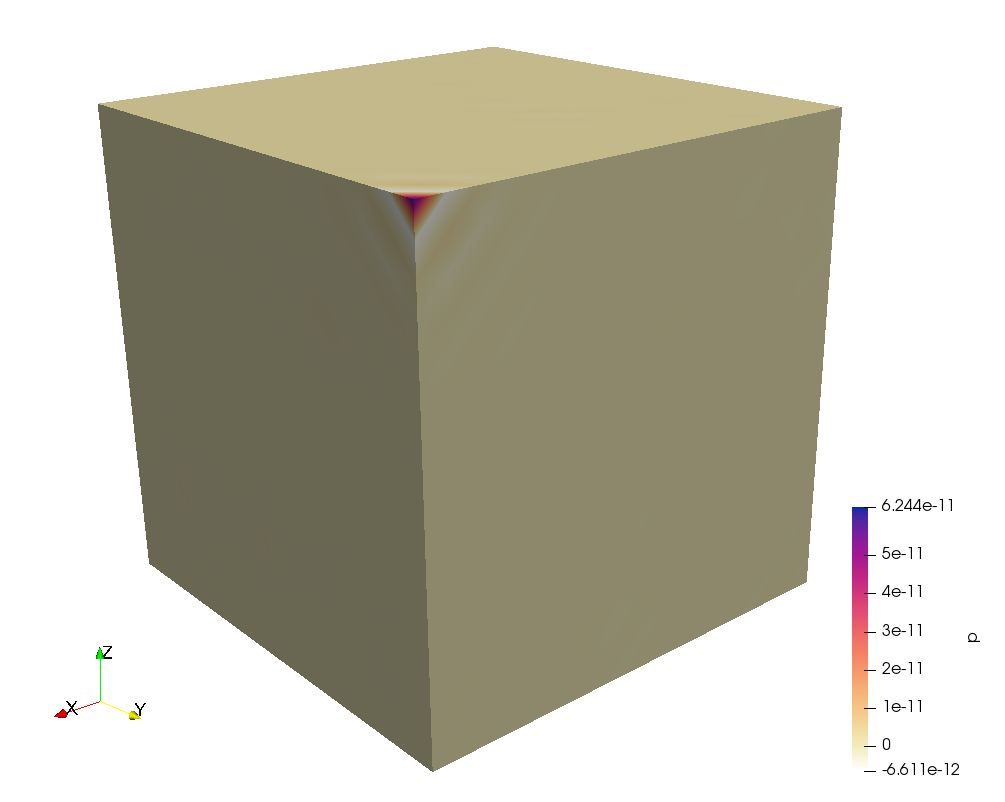
\includegraphics[width=5cm]{python_codes/fieldstone_82/RESULTS/bench2/press}\\
{\captionfont $20\times 20 \times 20$ mesh.} 
\end{center}


\begin{center}
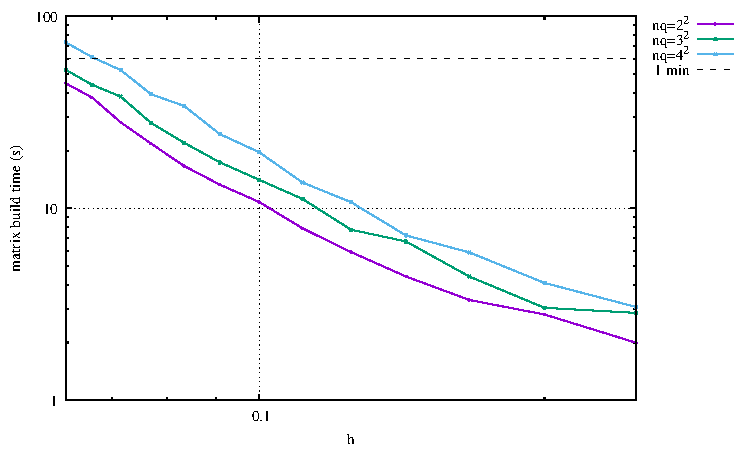
\includegraphics[width=8cm]{python_codes/fieldstone_82/RESULTS/bench2/build.pdf}
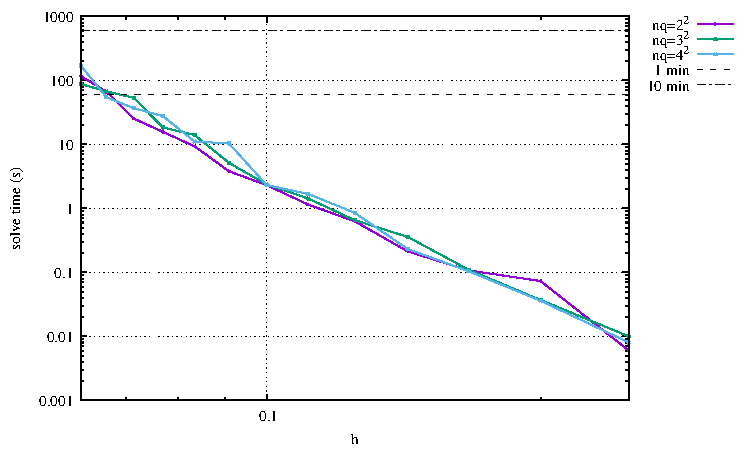
\includegraphics[width=8cm]{python_codes/fieldstone_82/RESULTS/bench2/solve.pdf}\\
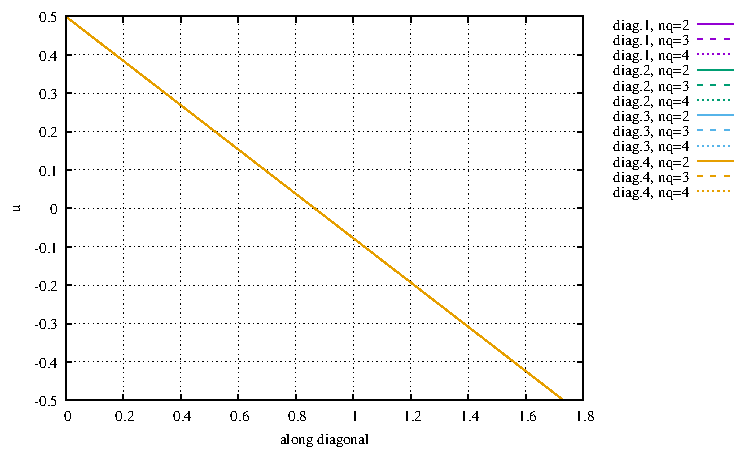
\includegraphics[width=5.7cm]{python_codes/fieldstone_82/RESULTS/bench2/diags_u.pdf}
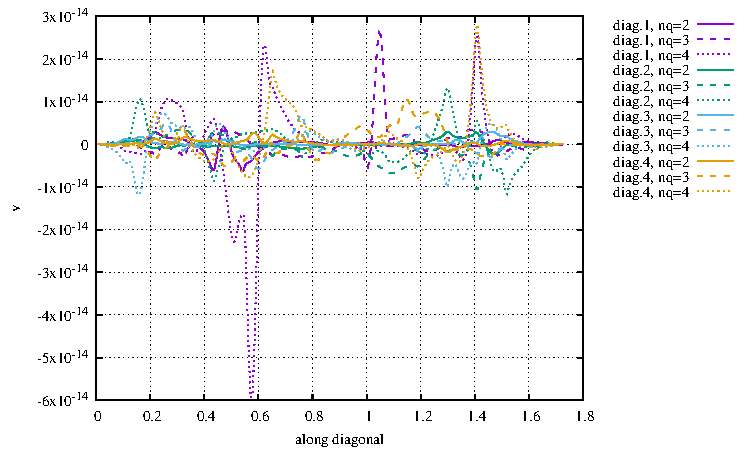
\includegraphics[width=5.7cm]{python_codes/fieldstone_82/RESULTS/bench2/diags_v.pdf}
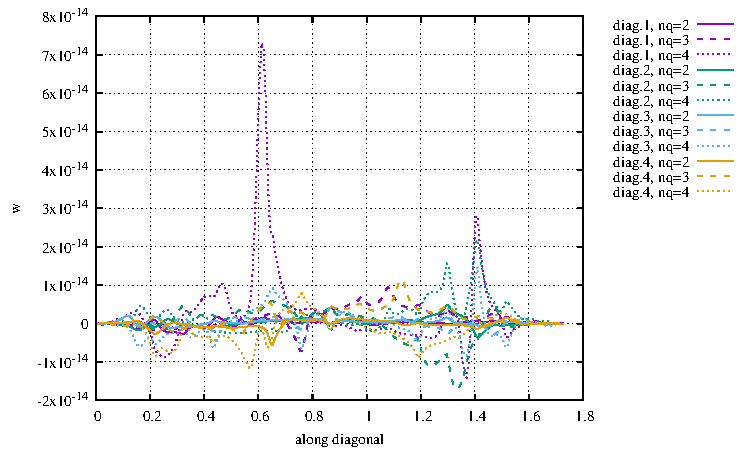
\includegraphics[width=5.7cm]{python_codes/fieldstone_82/RESULTS/bench2/diags_w.pdf}\\
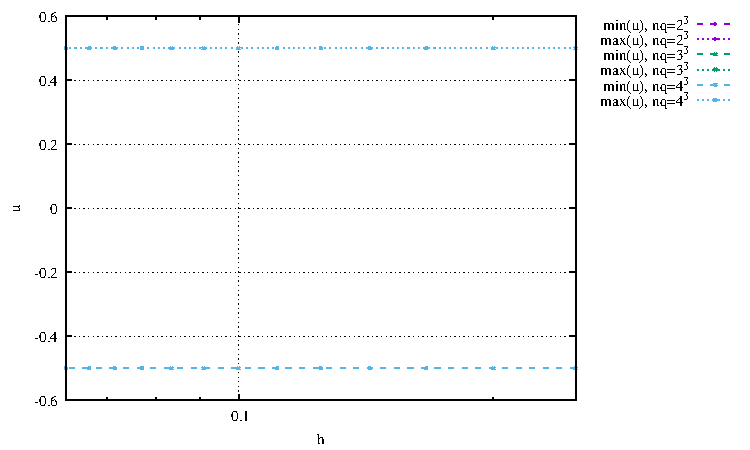
\includegraphics[width=5.7cm]{python_codes/fieldstone_82/RESULTS/bench2/u.pdf}
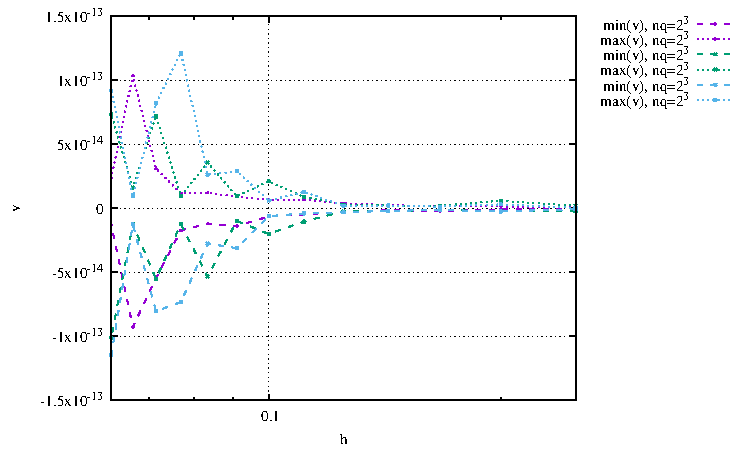
\includegraphics[width=5.7cm]{python_codes/fieldstone_82/RESULTS/bench2/v.pdf}
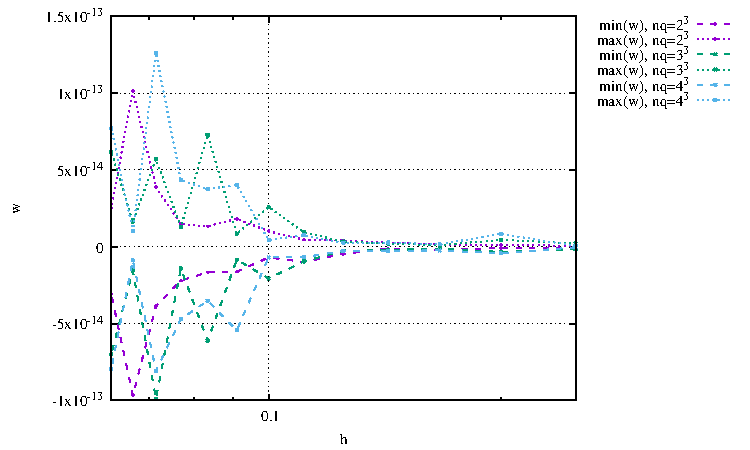
\includegraphics[width=5.7cm]{python_codes/fieldstone_82/RESULTS/bench2/w.pdf}\\
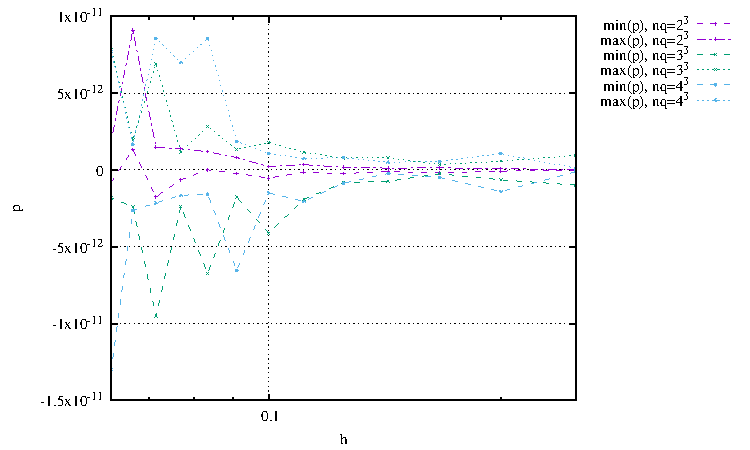
\includegraphics[width=5.7cm]{python_codes/fieldstone_82/RESULTS/bench2/p.pdf}
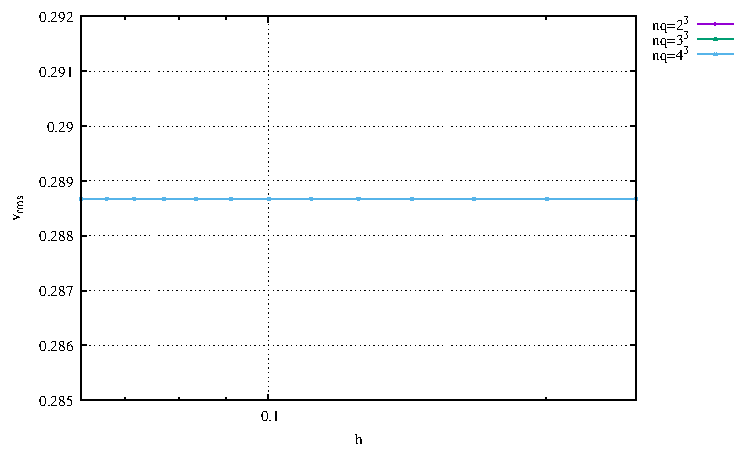
\includegraphics[width=5.7cm]{python_codes/fieldstone_82/RESULTS/bench2/vrms.pdf}
\end{center}










\newpage
%......................................
\subsection*{Stokes sphere ({\tt bench=3})}

This is the benchmark of Section~\ref{MMM-ss:stokes_sphere3D}.
A sphere of radius 0.123456789 is placed in the middle of the domain. 
It has a density excess $\delta\rho=0.01$
with respect to the surrounding fluid which has a density $\rho_{fluid}=1$. 
The sphere viscosity is 1000 while the fluid viscosity is 1.
Boundary conditions are no slip on all sides. Gravity is $\vec{g}=-\vec{e}_z$.

\begin{center}
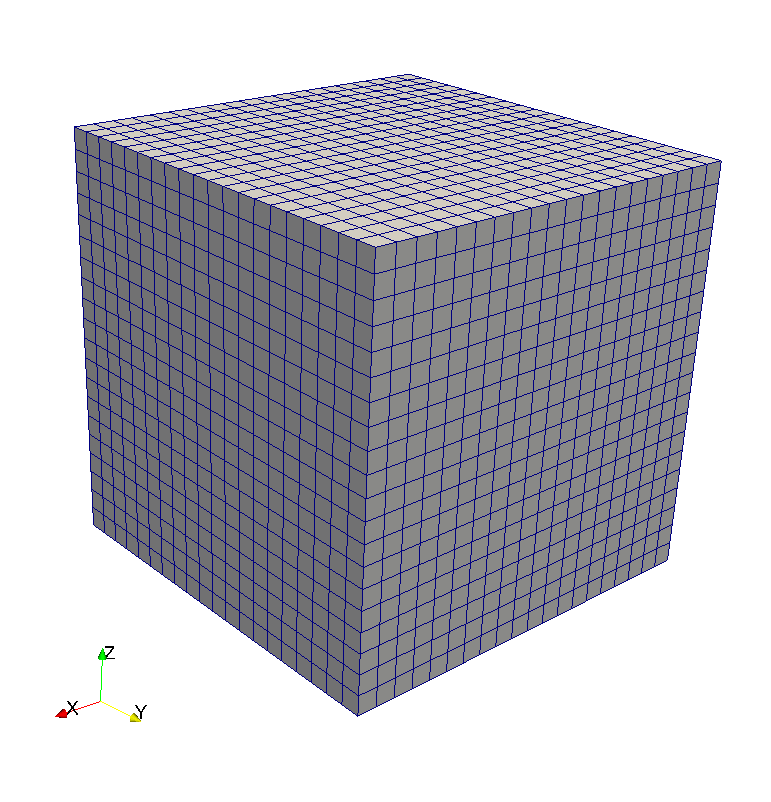
\includegraphics[width=5cm]{python_codes/fieldstone_82/RESULTS/bench3/grid.png}
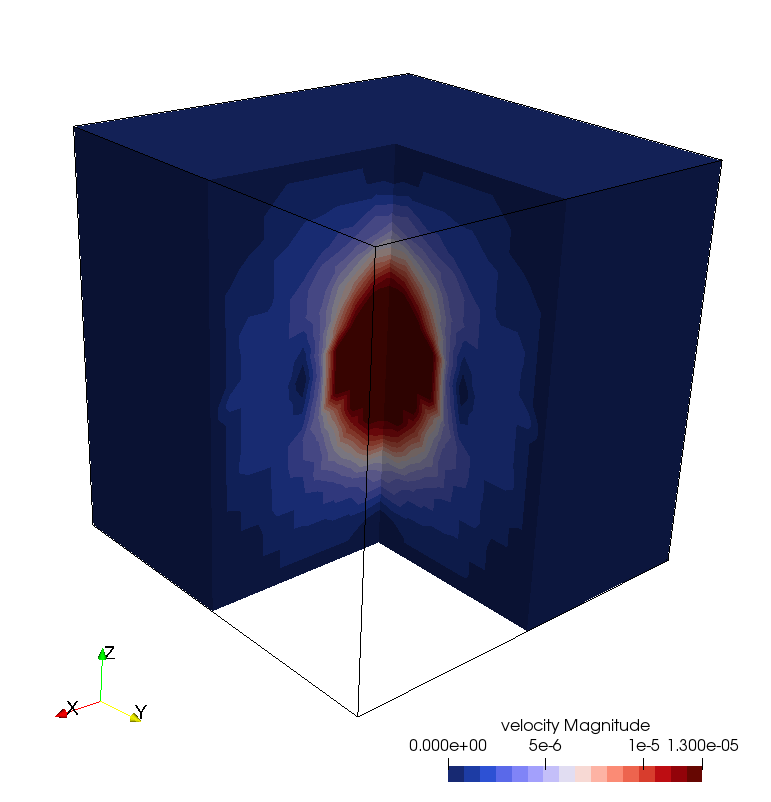
\includegraphics[width=5cm]{python_codes/fieldstone_82/RESULTS/bench3/vel.png}
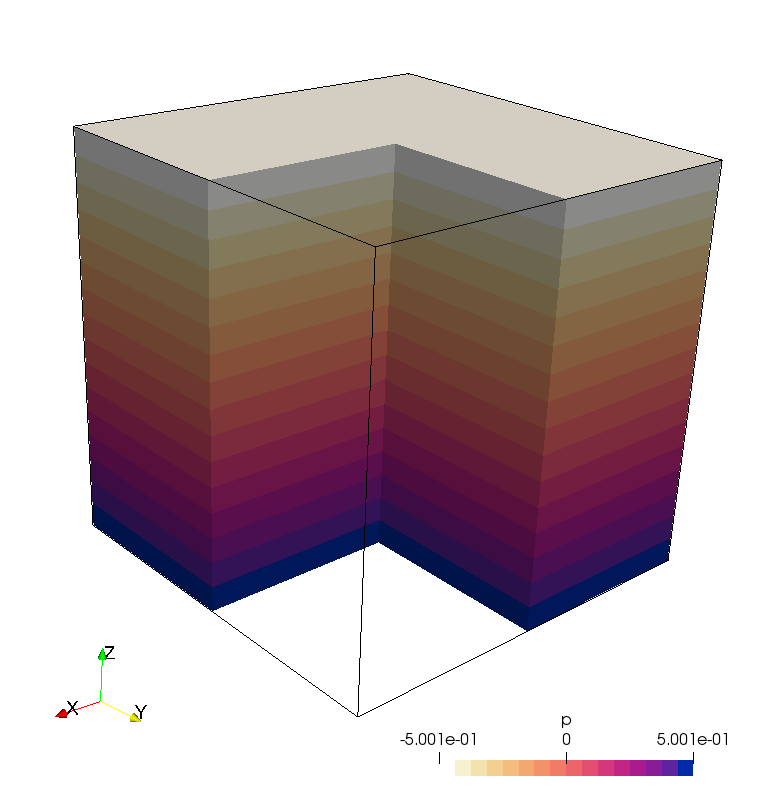
\includegraphics[width=5cm]{python_codes/fieldstone_82/RESULTS/bench3/press.png}\\
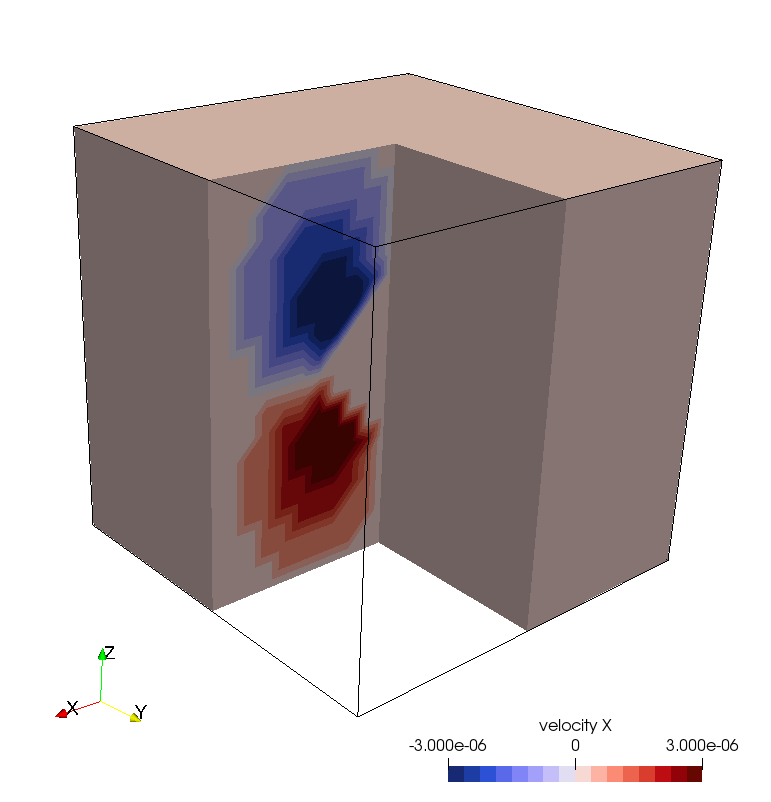
\includegraphics[width=5cm]{python_codes/fieldstone_82/RESULTS/bench3/u.png}
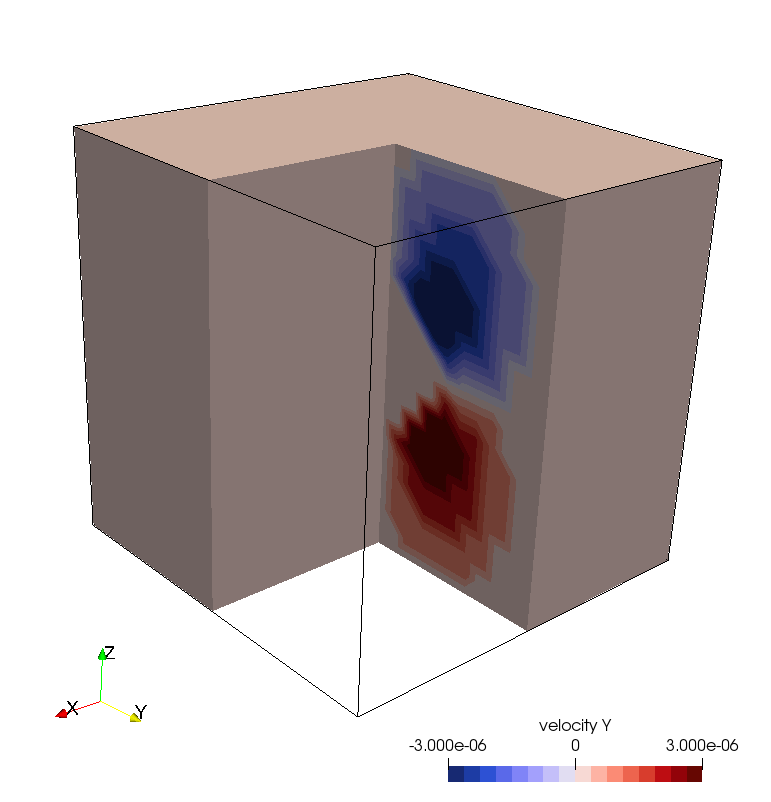
\includegraphics[width=5cm]{python_codes/fieldstone_82/RESULTS/bench3/v.png}
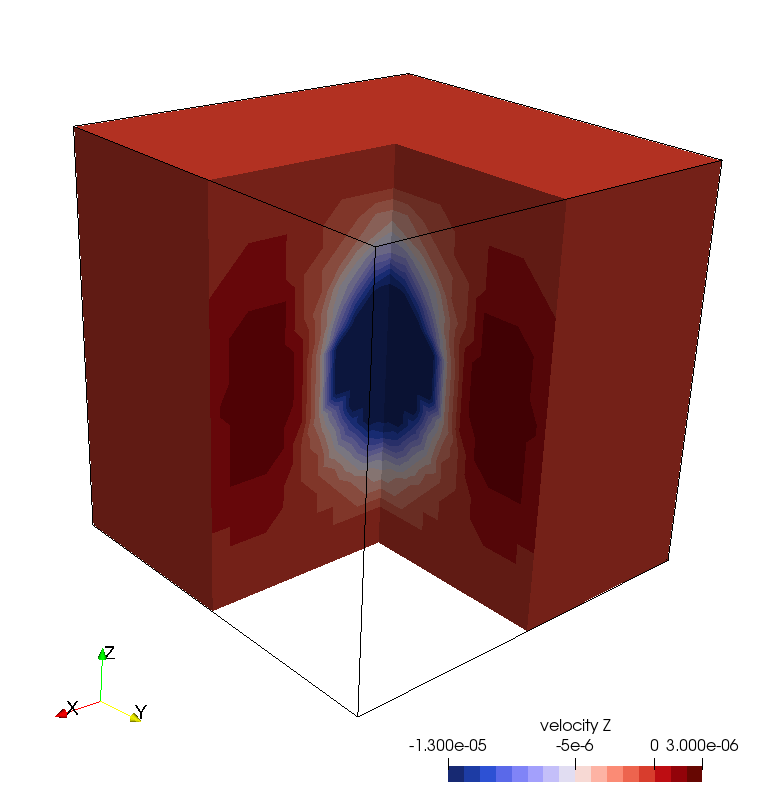
\includegraphics[width=5cm]{python_codes/fieldstone_82/RESULTS/bench3/w.png}\\
{\captionfont Resolution $20\times 20\times 20$. Quadrature $2\times 2 \times 2$.} 
\end{center}

All velocity and pressure statistics are presented in Section~\ref{MMM-ss:stokes_sphere3D}.

\begin{center}
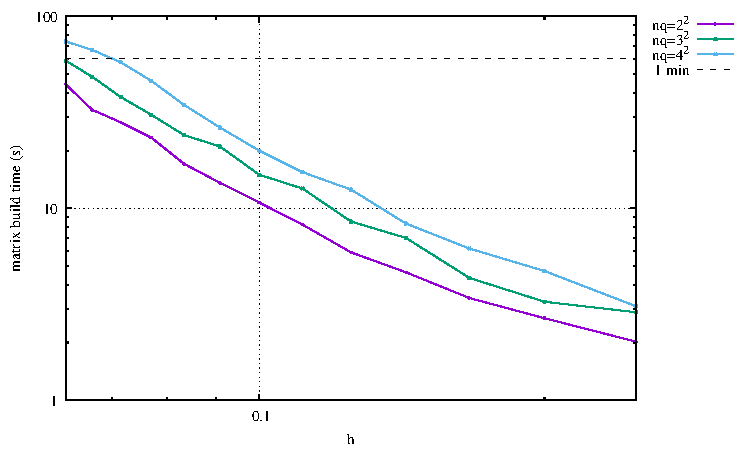
\includegraphics[width=8cm]{python_codes/fieldstone_82/RESULTS/bench3/build.pdf}
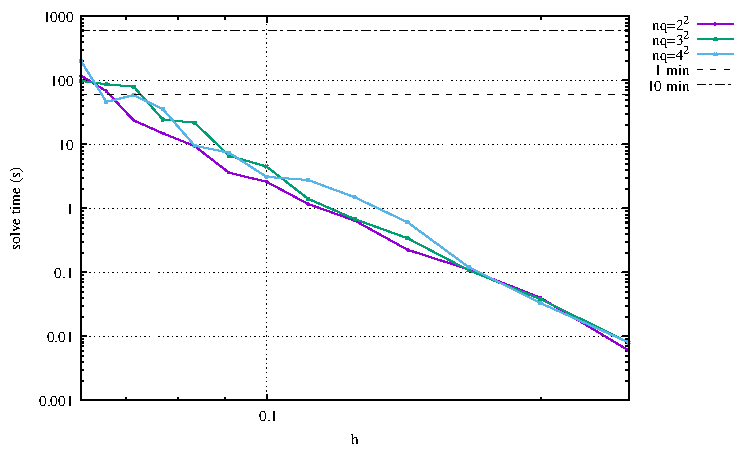
\includegraphics[width=8cm]{python_codes/fieldstone_82/RESULTS/bench3/solve.pdf}\\
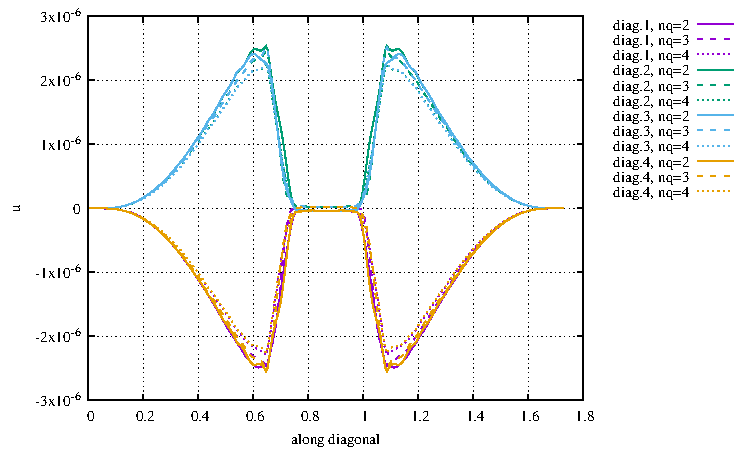
\includegraphics[width=5.7cm]{python_codes/fieldstone_82/RESULTS/bench3/diags_u.pdf}
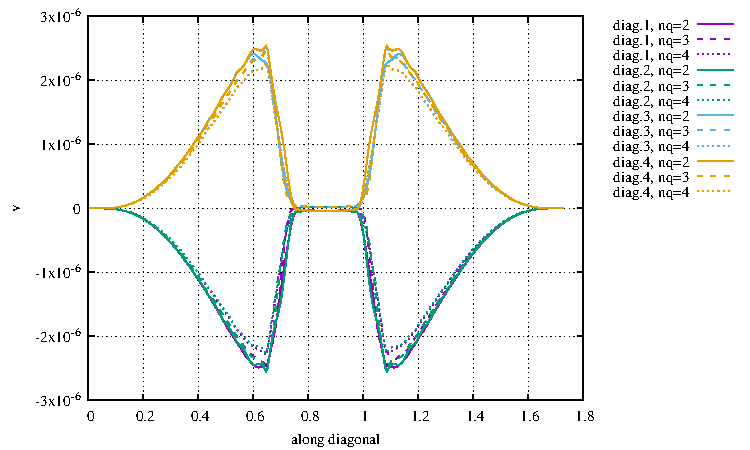
\includegraphics[width=5.7cm]{python_codes/fieldstone_82/RESULTS/bench3/diags_v.pdf}
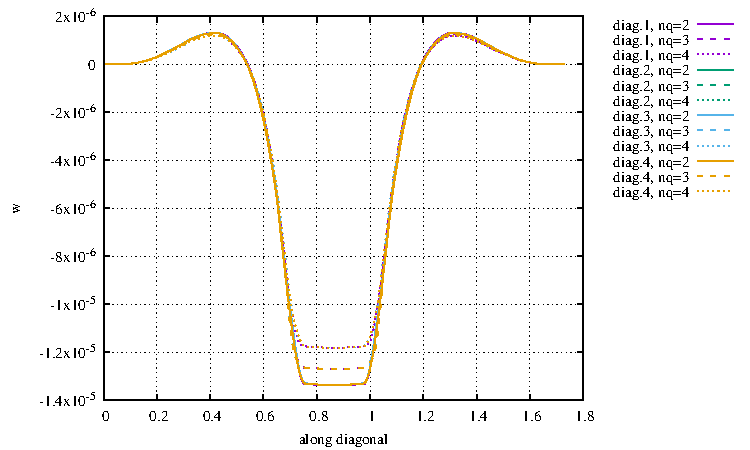
\includegraphics[width=5.7cm]{python_codes/fieldstone_82/RESULTS/bench3/diags_w.pdf}\\
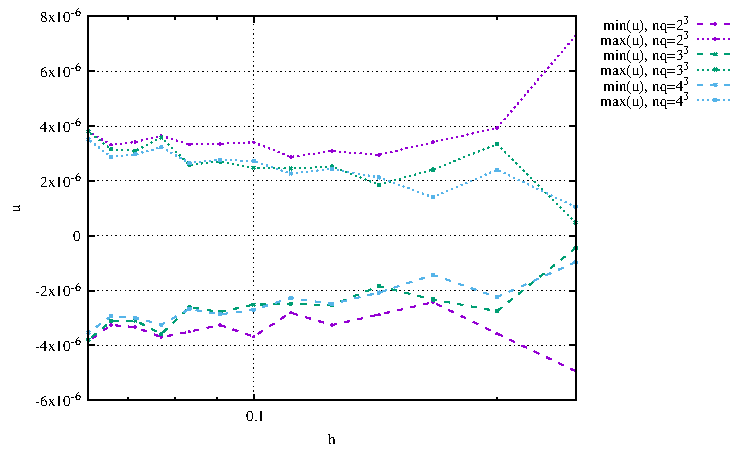
\includegraphics[width=5.7cm]{python_codes/fieldstone_82/RESULTS/bench3/u.pdf}
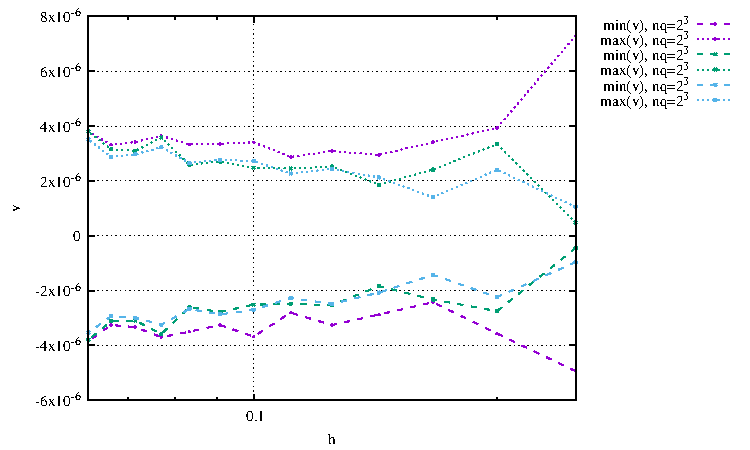
\includegraphics[width=5.7cm]{python_codes/fieldstone_82/RESULTS/bench3/v.pdf}
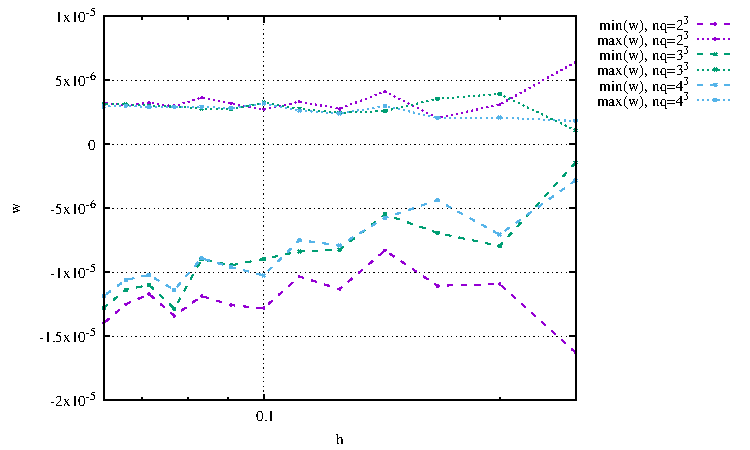
\includegraphics[width=5.7cm]{python_codes/fieldstone_82/RESULTS/bench3/w.pdf}
\end{center}







\newpage
%......................................
\subsection*{Sinking cube (bench=4)}

This is the same experiment as the Stokes sphere with the exception of the geometry of the sinker which 
is $0.25\times 0.25 \times 0.25$ in size so that its edges align with boundary edges 
for $8 \times 8 \times 8$, $16 \times 16 \times 16$ and $24 \times 24 \times 24$ meshes.
Reduced density is used in order to remove the lithostatic pressure signal.
 
\begin{center}
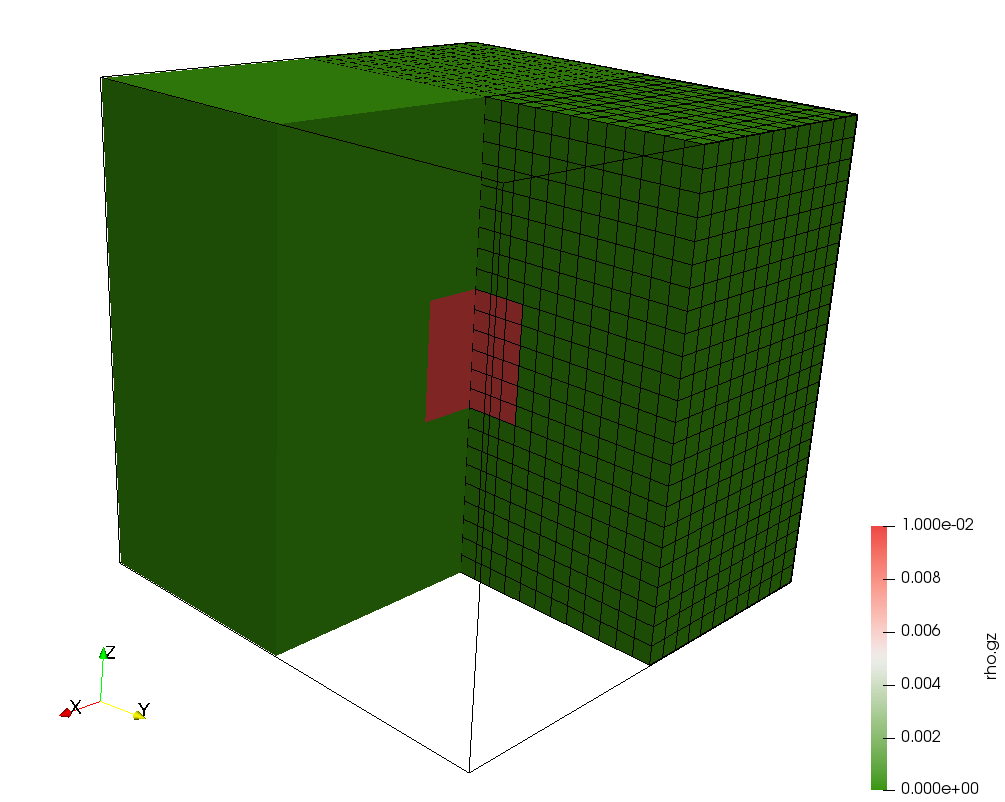
\includegraphics[width=8cm]{python_codes/fieldstone_82/RESULTS/bench4/rho}
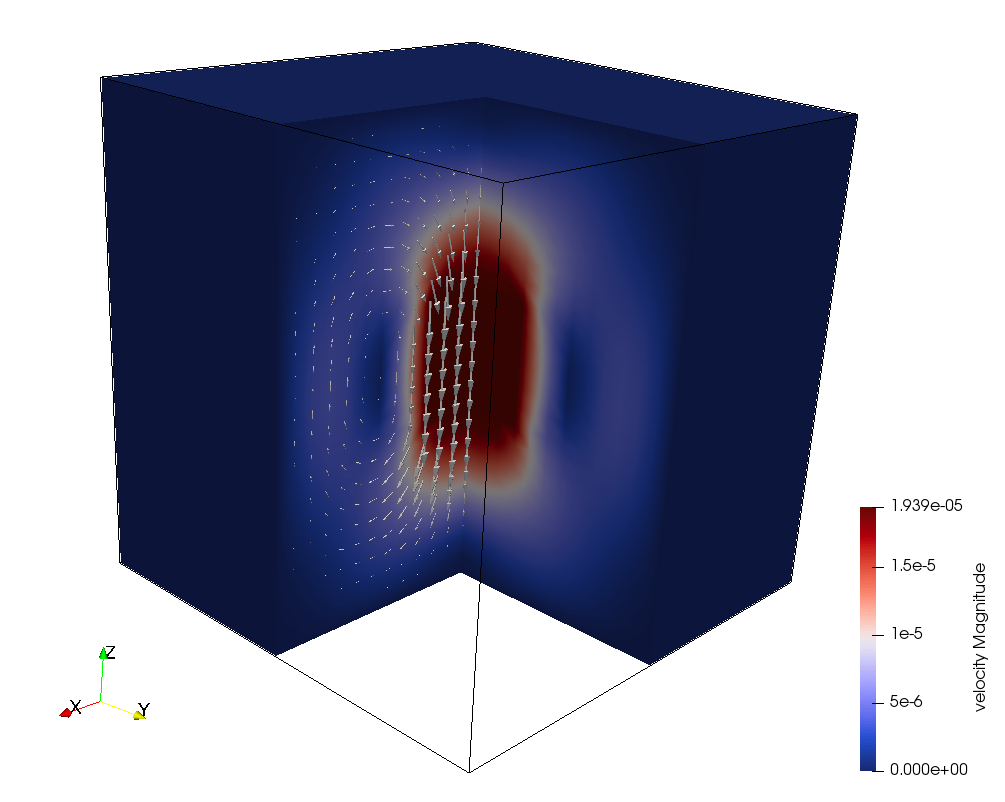
\includegraphics[width=8cm]{python_codes/fieldstone_82/RESULTS/bench4/vel}\\
{\captionfont resolution $24\times 24 \times 24$ elements.}
\end{center}

The velocity and pressures are interpolated on 100 points on the four diagonals of the cube
as a way to verify the symmetry of the solution (the bubbles rely on the basis 
functions of nodes 0 and 6 afterall!). $2^3$ quadrature points per element are used. 

\begin{center}
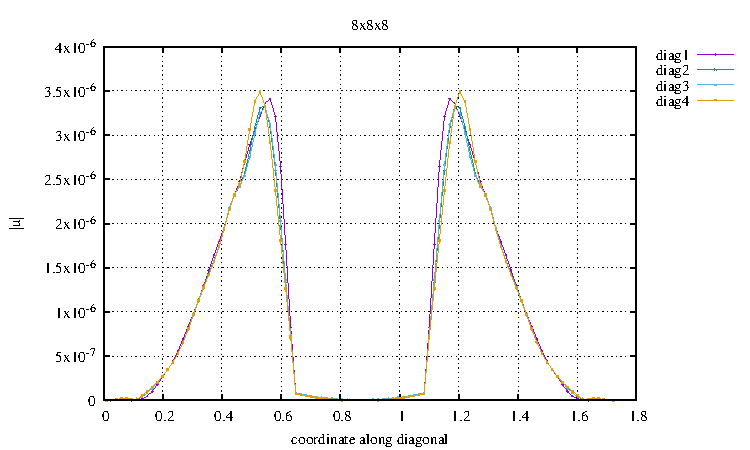
\includegraphics[width=5.5cm]{python_codes/fieldstone_82/RESULTS/bench4/u_08}
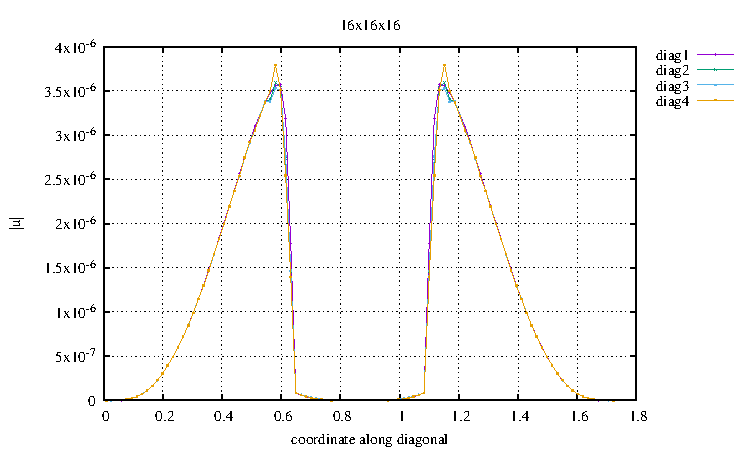
\includegraphics[width=5.5cm]{python_codes/fieldstone_82/RESULTS/bench4/u_16}
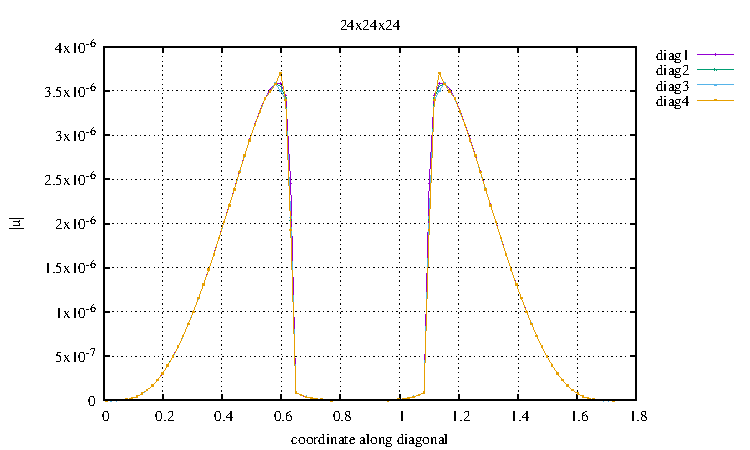
\includegraphics[width=5.5cm]{python_codes/fieldstone_82/RESULTS/bench4/u_24}\\
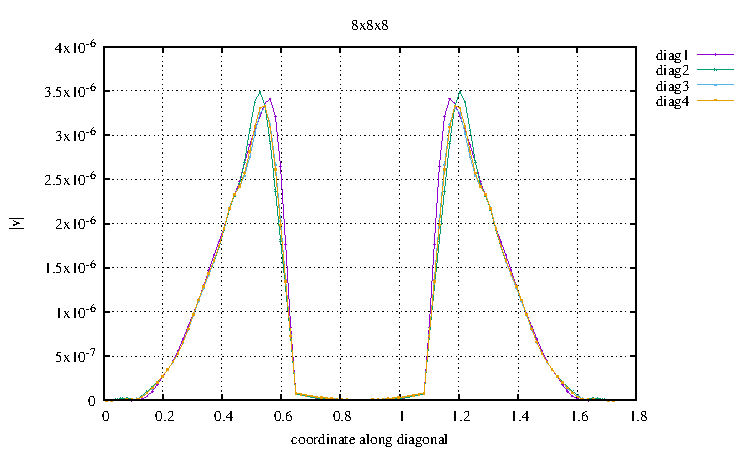
\includegraphics[width=5.5cm]{python_codes/fieldstone_82/RESULTS/bench4/v_08}
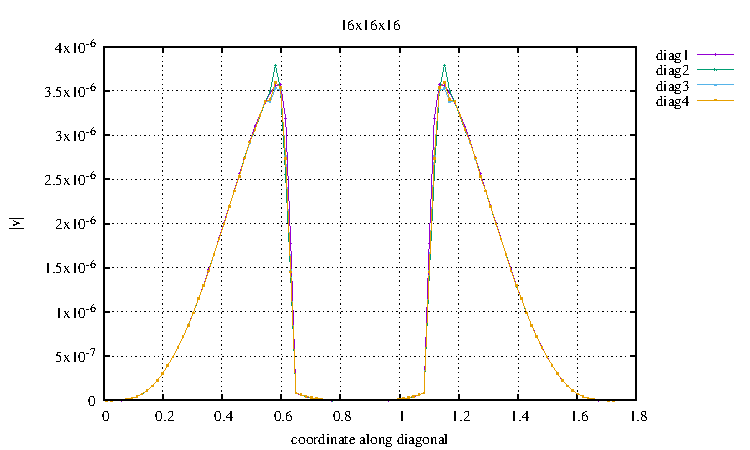
\includegraphics[width=5.5cm]{python_codes/fieldstone_82/RESULTS/bench4/v_16}
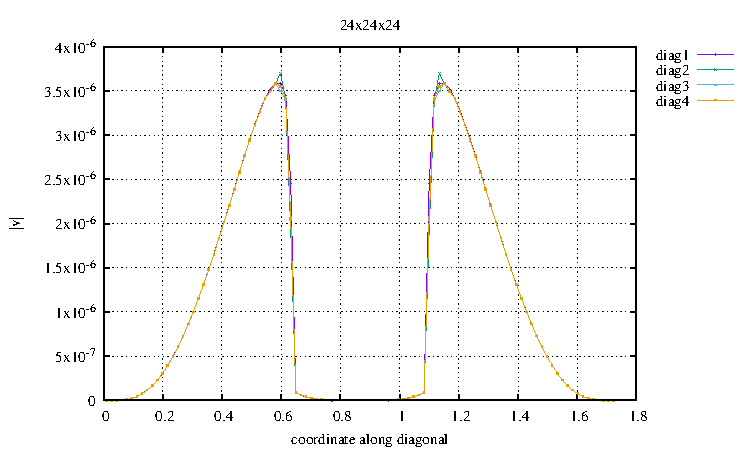
\includegraphics[width=5.5cm]{python_codes/fieldstone_82/RESULTS/bench4/v_24}\\
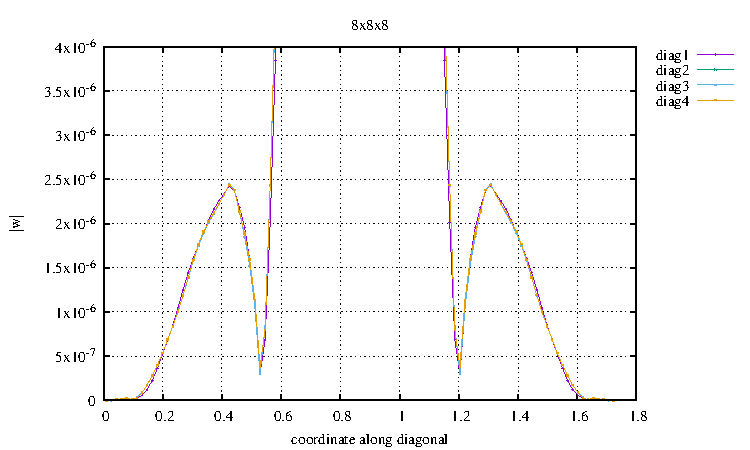
\includegraphics[width=5.5cm]{python_codes/fieldstone_82/RESULTS/bench4/w_08}
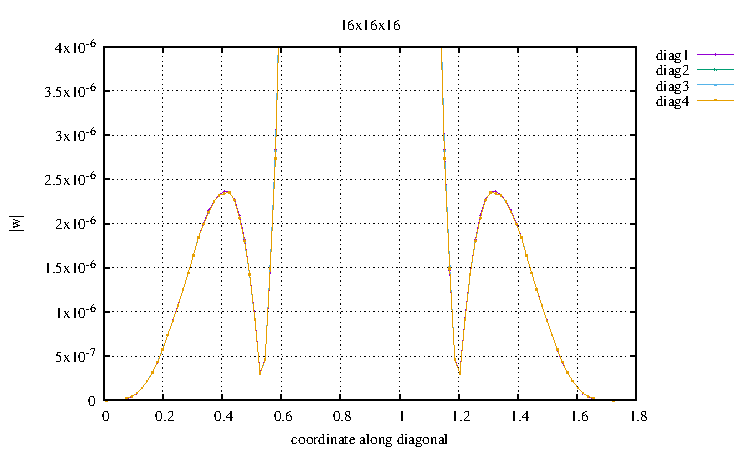
\includegraphics[width=5.5cm]{python_codes/fieldstone_82/RESULTS/bench4/w_16}
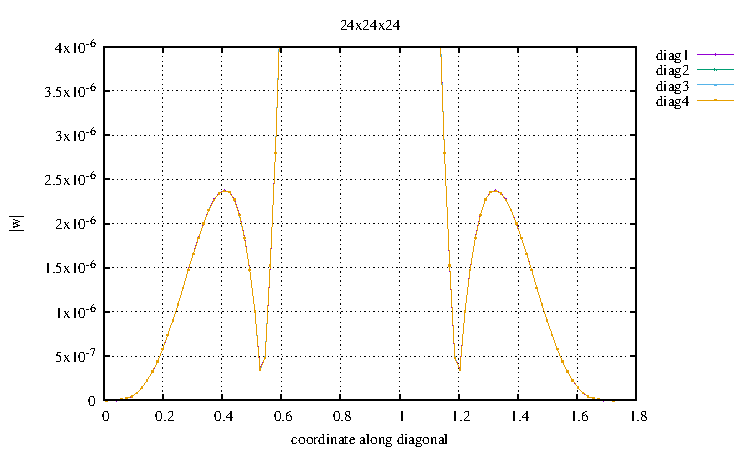
\includegraphics[width=5.5cm]{python_codes/fieldstone_82/RESULTS/bench4/w_24}\\
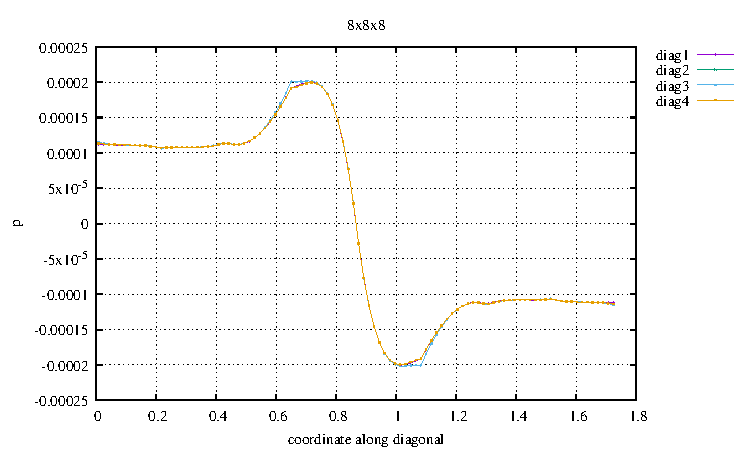
\includegraphics[width=5.5cm]{python_codes/fieldstone_82/RESULTS/bench4/p_08}
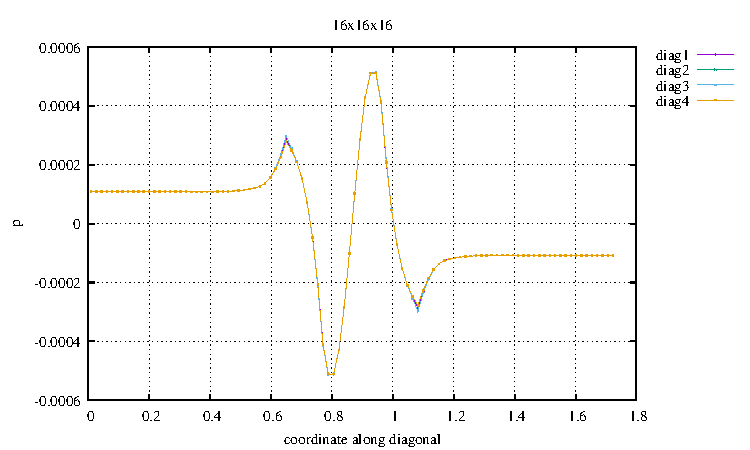
\includegraphics[width=5.5cm]{python_codes/fieldstone_82/RESULTS/bench4/p_16}
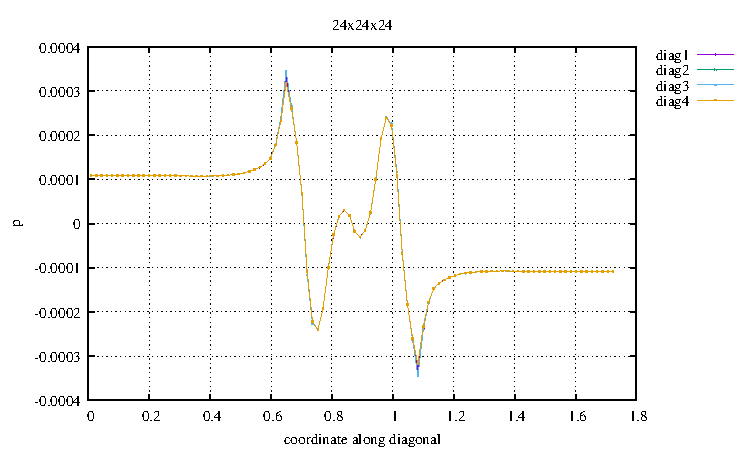
\includegraphics[width=5.5cm]{python_codes/fieldstone_82/RESULTS/bench4/p_24}\\
{\captionfont Left to right: increasing resolution}
\end{center}

We can also plot the velocity and pressure fields on a vertical line passing 
through the middle of the block:
\begin{center}
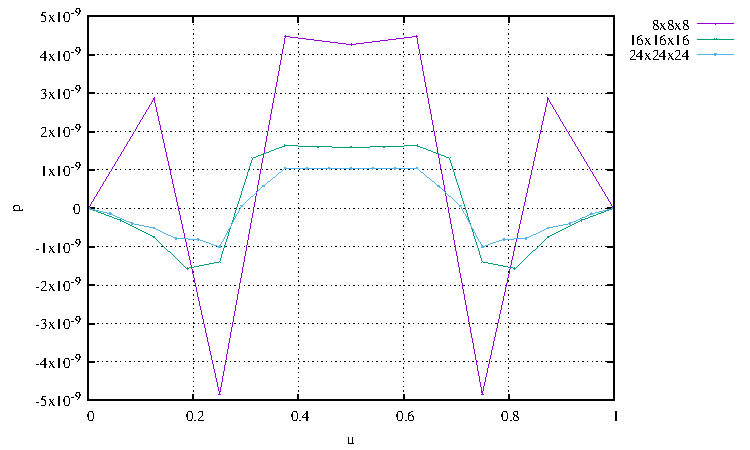
\includegraphics[width=5.5cm]{python_codes/fieldstone_82/RESULTS/bench4/vert_u}
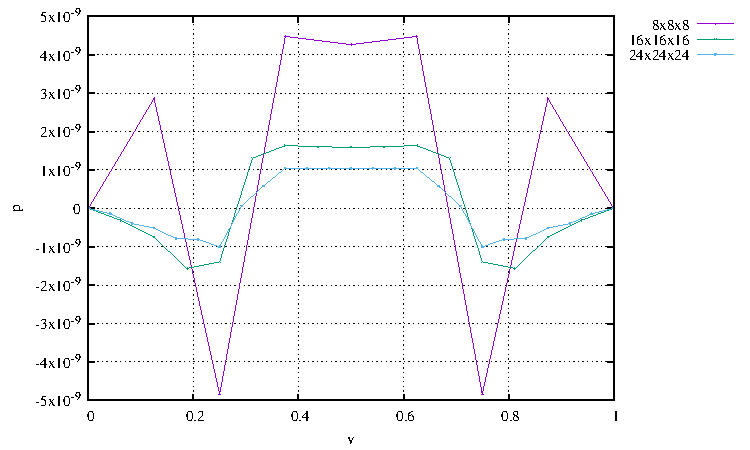
\includegraphics[width=5.5cm]{python_codes/fieldstone_82/RESULTS/bench4/vert_v}
\includegraphics[width=5.5cm]{python_codes/fieldstone_82/RESULTS/bench4/vert_w}
\includegraphics[width=5.5cm]{python_codes/fieldstone_82/RESULTS/bench4/vert_p}
\end{center}
We see that unfortunately the resolution $24\times 24 \times 24$ is most certainly not high 
enough to speak of capturing the true solution of the problem...

Also, one can verify that the solution is symmetric by looking at the averages of the 
velocity components (and their absolute value) as a function of the mesh size:
\begin{center}
\includegraphics[width=6cm]{python_codes/fieldstone_82/RESULTS/bench4/averages.pdf}
\includegraphics[width=6cm]{python_codes/fieldstone_82/RESULTS/bench4/averages_abs.pdf}
\end{center}
It seems that the somewhat anisotropic placement of the bubbles does not introduce 
a form of asymmetry in the solution.

\begin{center}
\includegraphics[width=8cm]{python_codes/fieldstone_82/RESULTS/bench4/build.pdf}
\includegraphics[width=8cm]{python_codes/fieldstone_82/RESULTS/bench4/solve.pdf}\\
\includegraphics[width=5.7cm]{python_codes/fieldstone_82/RESULTS/bench4/diags_u.pdf}
\includegraphics[width=5.7cm]{python_codes/fieldstone_82/RESULTS/bench4/diags_v.pdf}
\includegraphics[width=5.7cm]{python_codes/fieldstone_82/RESULTS/bench4/diags_w.pdf}\\
\includegraphics[width=5.7cm]{python_codes/fieldstone_82/RESULTS/bench4/u.pdf}
\includegraphics[width=5.7cm]{python_codes/fieldstone_82/RESULTS/bench4/v.pdf}
\includegraphics[width=5.7cm]{python_codes/fieldstone_82/RESULTS/bench4/w.pdf}\\
\includegraphics[width=5.7cm]{python_codes/fieldstone_82/RESULTS/bench4/p.pdf}
\includegraphics[width=5.7cm]{python_codes/fieldstone_82/RESULTS/bench4/vrms.pdf}
\end{center}






\newpage
%......................................
\subsection*{Manufactured solution (bench=5)}

We here consider the manufactured solution which is introduced 
in Section~\ref{MMM-ss:mms3Dgen}. The velocity and pressure fields are
given by:
\begin{eqnarray}
u(x,y,z) &=& x(1-x)(1-2y)(1-2z) \nn\\
v(x,y,z) &=& (1-2x) y(1-y) (1-2z) \nn\\
w(x,y,z) &=& -2(1-2x)(1-2y)z(1-z) \nn\\
p(x,y,z) &=& (2x-1)(2y-1)(2z-1) \nn
\end{eqnarray}
This flow field has the built-in property that there is no flux through the 
boundaries:

\begin{center}
\includegraphics[width=5.2cm]{python_codes/fieldstone_82/RESULTS/bench5/vel1}
\includegraphics[width=5.2cm]{python_codes/fieldstone_82/RESULTS/bench5/vel2}
\includegraphics[width=5.2cm]{python_codes/fieldstone_82/RESULTS/bench5/velth}\\
\includegraphics[width=5.2cm]{python_codes/fieldstone_82/RESULTS/bench5/press1}
\includegraphics[width=5.2cm]{python_codes/fieldstone_82/RESULTS/bench5/press2}
\includegraphics[width=5.2cm]{python_codes/fieldstone_82/RESULTS/bench5/pressth}
\end{center}

We can look at the root mean square velocity and the velocity and pressure errors:

\begin{center}
\includegraphics[width=8cm]{python_codes/fieldstone_82/RESULTS/bench5/vrms.pdf}
\includegraphics[width=8cm]{python_codes/fieldstone_82/RESULTS/bench5/conv.pdf}\\
{\captionfont Results obtained for three levels of quadrature. The velocity error 
convergence is quadratic but the pressure seems to converge like $h^{1.6}$.
Also the errors are the smallest for $nq=2^3$.}
\end{center}

When using the Preconditioned Conjugate Gradients algorithm on the Schur complement 
we find that the number of iterations is constant across the range of resolutions
that can be used:

\begin{center}
\includegraphics[width=8cm]{python_codes/fieldstone_82/RESULTS/bench5/solver_convergence.pdf}
\end{center}

\begin{center}
\includegraphics[width=5.7cm]{python_codes/fieldstone_82/RESULTS/bench5/build.pdf}
\includegraphics[width=5.7cm]{python_codes/fieldstone_82/RESULTS/bench5/solve.pdf}
\includegraphics[width=5.7cm]{python_codes/fieldstone_82/RESULTS/bench5/p.pdf}
\includegraphics[width=5.7cm]{python_codes/fieldstone_82/RESULTS/bench5/diags_u.pdf}
\includegraphics[width=5.7cm]{python_codes/fieldstone_82/RESULTS/bench5/diags_v.pdf}
\includegraphics[width=5.7cm]{python_codes/fieldstone_82/RESULTS/bench5/diags_w.pdf}\\
\includegraphics[width=5.7cm]{python_codes/fieldstone_82/RESULTS/bench5/u.pdf}
\includegraphics[width=5.7cm]{python_codes/fieldstone_82/RESULTS/bench5/v.pdf}
\includegraphics[width=5.7cm]{python_codes/fieldstone_82/RESULTS/bench5/w.pdf}\\
\end{center}







\newpage
%..............................................................................
\subsection*{bench=-1: computing Ker($\G$) on a $2\times 2 \times 2$ mesh}

We consider a mesh composed of $2\times 2\times 2$ elements. We prescribe no slip boundary conditions 
on all sides, so that only the node in the middle has 3 velocity dofs left, in addition 
to the 8*2=16 bubbles counting in total 48 velocity dofs, so 51 vdofs are left.

The matrix $\G$ is [(3*3*3)+(8*2)]*3=43*3=129 vdofs X (3*3*3=27) pdofs. 
Imposing the boundary conditions will zero 26*3=78 lines so that the leftover matrix $\G$
has size $51\times 27$. If this element is stable its nullspace should be of size 1. 

Given the ordering of the nodes, the middle node has global number 13, so that 
its vdofs are 39, 40, and 41. The bubbles occupy rows 81 to 128. 
We create a matrix $\G_2$ which contains only the lines of $\G$ which contain non-zero terms:
\begin{lstlisting}
G2 = np.zeros((51,NfemP),dtype=np.float64)
G2[0:3,:]=G_mat[39:42,:] 
G2[3:,:]=G_mat[81:,:]    
\end{lstlisting}
We then proceed to find the kernel/nullspace of matrix $\G_2$:
\begin{lstlisting}
ns = null_space(G2)
\end{lstlisting}
and we find that its size is just 1, as expected. 


